\documentclass[tikz, border=12pt]{standalone}
\usepackage{tikz}
\usepackage{amsmath}
\usepackage{amssymb}
\usetikzlibrary{arrows.meta, positioning, fit, backgrounds, calc}

\definecolor{cpuBlue}{RGB}{180,210,240}
\definecolor{cpuPurple}{RGB}{200,190,240}
\definecolor{cpuCoral}{RGB}{240,180,165}
\definecolor{cpuAmber}{RGB}{250,220,160}
\definecolor{cpuTeal}{RGB}{160,225,205}
\definecolor{cpuGray}{RGB}{220,218,210}
\definecolor{bdGray}{RGB}{140,138,130}
\definecolor{shBg}{RGB}{250,249,246}

\tikzset{
  wide/.style={rectangle, rounded corners=5pt,
    text width=12.5cm, minimum height=1.05cm,
    draw=bdGray, line width=0.4pt, font=\small, align=center},
  blueN/.style={wide, fill=cpuBlue, text width=5.8cm},
  tealN/.style={wide, fill=cpuTeal},
  tealS/.style={wide, fill=cpuTeal, text width=5.8cm},
  purpleN/.style={wide, fill=cpuPurple},
  coralN/.style={wide, fill=cpuCoral, minimum height=1.5cm, line width=0.8pt},
  amberN/.style={wide, fill=cpuAmber},
  grayN/.style={wide, fill=cpuGray, text width=3.8cm},
  dispN/.style={wide, fill=cpuTeal, minimum height=1.6cm},
  platN/.style={wide, fill=shBg, draw=bdGray!55, dashed, minimum height=1.05cm},
  arr/.style={-{Stealth[length=5pt,width=4pt]}, line width=0.7pt, color=bdGray},
  blueArr/.style={-{Stealth[length=5pt,width=4pt]}, line width=1.0pt, color=cpuBlue!70!black},
  slabel/.style={font=\footnotesize\itshape, text=bdGray},
  clabel/.style={font=\ttfamily\footnotesize, text=bdGray!80},
}

\begin{document}
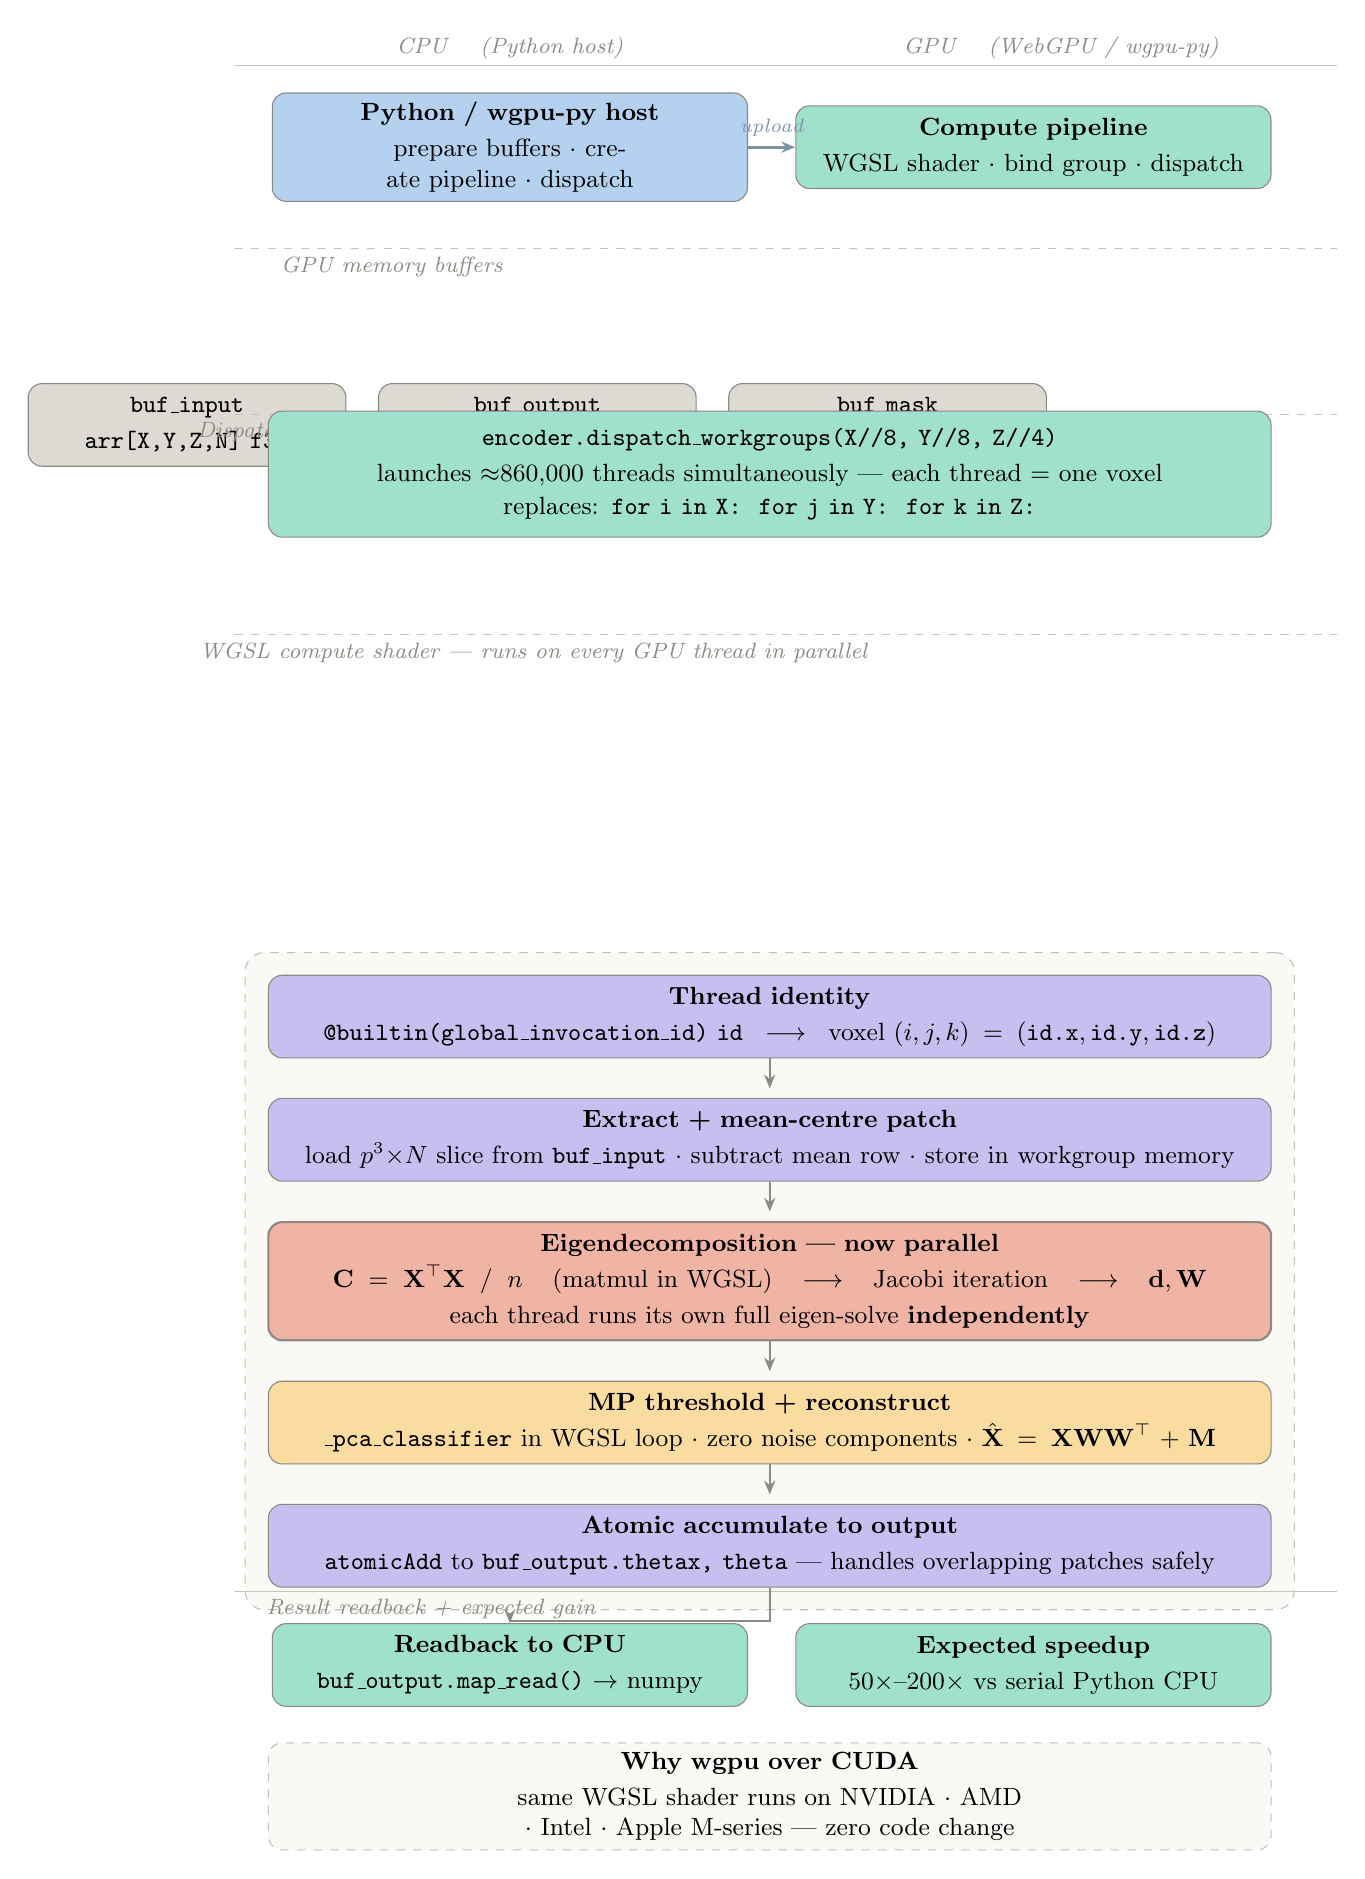
\begin{tikzpicture}[node distance=0.45cm and 0.5cm]

%% ── HEADERS ─────────────────────────────────────────────
\node[slabel] (Lc) at (-3.5,0) {CPU \quad (Python host)};
\node[slabel] (Lg) at ( 3.5,0) {GPU \quad (WebGPU / wgpu-py)};
\draw[bdGray!50, line width=0.3pt] (-7.0,-0.22) -- (7.0,-0.22);

\node[blueN, below=0.3cm of Lc, xshift=0] (host)
  {\textbf{Python / wgpu-py host}\\[2pt]
   prepare buffers $\cdot$ create pipeline $\cdot$ dispatch};

\node[tealS, right=0.6cm of host] (pip)
  {\textbf{Compute pipeline}\\[2pt]
   WGSL shader $\cdot$ bind group $\cdot$ dispatch};

\draw[blueArr] (host.east) -- node[above,font=\scriptsize\itshape]{upload} (pip.west);

%% ── BUFFERS ─────────────────────────────────────────────
\draw[bdGray!50, dashed, line width=0.3pt] (-7.0,-2.55) -- (7.0,-2.55);
\node[slabel] at (-5.0,-2.78) {GPU memory buffers};

\node[grayN, below=2.3cm of host, xshift=-4.1cm] (B1)
  {\textbf{\texttt{buf\_input}}\\[2pt]\texttt{arr[X,Y,Z,N] f32}};
\node[grayN, right=0.4cm of B1] (B2)
  {\textbf{\texttt{buf\_output}}\\[2pt]\texttt{thetax, theta f32}};
\node[grayN, right=0.4cm of B2] (B3)
  {\textbf{\texttt{buf\_mask}}\\[2pt]\texttt{mask[X,Y,Z] u32}};

%% ── DISPATCH ─────────────────────────────────────────────
\draw[bdGray!50, dashed, line width=0.3pt] (-7.0,-4.65) -- (7.0,-4.65);
\node[slabel] at (-3.0,-4.88)
  {Dispatch --- one thread per voxel \quad (replaces the triple Python loop)};

\node[dispN, below=2.65cm of host, xshift=3.3cm] (disp)
  {\textbf{\texttt{encoder.dispatch\_workgroups(X//8,\ Y//8,\ Z//4)}}\\[2pt]
   launches ${\approx}860{,}000$ threads simultaneously --- each thread $=$ one voxel\\[1pt]
   replaces: \texttt{for i in X:\ \ for j in Y:\ \ for k in Z:}};

%% ── WGSL SHADER ─────────────────────────────────────────
\draw[bdGray!50, dashed, line width=0.3pt] (-7.0,-7.45) -- (7.0,-7.45);
\node[slabel] at (-3.2,-7.68)
  {WGSL compute shader --- runs on every GPU thread in parallel};

\node[purpleN, below=5.55cm of disp] (T1)
  {\textbf{Thread identity}\\[2pt]
   \texttt{@builtin(global\_invocation\_id) id}
   $\;\longrightarrow\;$ voxel $(i,j,k) = (\texttt{id.x},\texttt{id.y},\texttt{id.z})$};
\draw[arr] (T1.south) -- ++(0,-0.38);

\node[purpleN, below=0.5cm of T1] (T2)
  {\textbf{Extract + mean-centre patch}\\[2pt]
   load $p^3{\times}N$ slice from \texttt{buf\_input}
   $\cdot$ subtract mean row
   $\cdot$ store in workgroup memory};
\draw[arr] (T2.south) -- ++(0,-0.38);

\node[coralN, below=0.5cm of T2] (T3)
  {\textbf{Eigendecomposition --- now parallel}\\[2pt]
   $\mathbf{C} = \mathbf{X}^\top\mathbf{X}\;/\;n \;\;\text{(matmul in WGSL)}
   \;\longrightarrow\; \text{Jacobi iteration}
   \;\longrightarrow\; \mathbf{d},\mathbf{W}$\\[2pt]
   each thread runs its own full eigen-solve \textbf{independently}};
\draw[arr] (T3.south) -- ++(0,-0.38);

\node[amberN, below=0.5cm of T3] (T4)
  {\textbf{MP threshold + reconstruct}\\[2pt]
   \texttt{\_pca\_classifier} in WGSL loop
   $\cdot$ zero noise components
   $\cdot$ $\hat{\mathbf{X}} = \mathbf{X}\mathbf{W}\mathbf{W}^\top + \mathbf{M}$};
\draw[arr] (T4.south) -- ++(0,-0.38);

\node[purpleN, below=0.5cm of T4] (T5)
  {\textbf{Atomic accumulate to output}\\[2pt]
   \texttt{atomicAdd} to \texttt{buf\_output.thetax, theta}
   --- handles overlapping patches safely};

\begin{pgfonlayer}{background}
  \node[draw=bdGray!55, dashed, fill=shBg, rounded corners=7pt, inner sep=8pt,
        fit=(T1)(T2)(T3)(T4)(T5)] (shbox) {};
\end{pgfonlayer}

%% ── READBACK ─────────────────────────────────────────────
\draw[bdGray!50, line width=0.3pt] (-7.0,-19.6) -- (7.0,-19.6);
\node[slabel] at (-4.5,-19.82) {Result readback + expected gain};

\node[tealS, below=0.45cm of T5, xshift=-3.3cm] (RB)
  {\textbf{Readback to CPU}\\[2pt]
   \texttt{buf\_output.map\_read()} $\rightarrow$ numpy};

\node[tealS, right=0.6cm of RB] (SP)
  {\textbf{Expected speedup}\\[2pt]
   $50{\times}$--$200{\times}$ vs serial Python CPU};

\draw[arr] (T5.south) -- ++(0,-0.42) -| (RB.north);

%% ── CROSS-PLATFORM NOTE ─────────────────────────────────
\node[platN, below=0.45cm of RB, xshift=3.3cm] (XP)
  {\textbf{Why wgpu over CUDA}\\[2pt]
   same WGSL shader runs on NVIDIA $\cdot$ AMD $\cdot$ Intel $\cdot$ Apple M-series --- zero code change};

\end{tikzpicture}
\end{document}
